\clearpage
\section{Technische Grundlagen Zigbee}\label{sec:TechnischeGrundlagenZigbee}

\subsection{Netzaufbau und Topologie}\label{subsec:ZigbeeNetzaufbauundTopologie}
Zigbee ist nicht gleich Zigbee.
Obschon Zigbee von einer zentralen Stelle der Zigbee Alliance spezifiziert wurde, gibt es eine Vielzahl an Versionen und Umsetzungsvarianten.
In den Spezifikationen der Zigbee Alliance wird zwischen zwei sogenannten Stackprofilen \textit{ZigBee} und \textit{ZigBee PRO} unterschieden.
Während \textit{ZigBee}-Netzwerke eine Baumstruktur bilden und der Koordinator dabei einen Single-Point-of-Failure darstellt, haben \textit{ZigBee PRO}-Netzwerke geroutete Mesh Funktionalitäten mit Routing Tabellen und Wegentdeckung.
Der Koordinator bildet dabei nicht länger einen Single-Point-of-Failure, da sich das Routing dynamisch anpassen kann.
Abbildung \ref{fig:NetzwerktopologienZigbee} zeigt die Unterschiede eines Baumnetzwerks im Stackprofil \textit{ZigBee} links, und eines Meshnetzwerks im Stackprofil \textit{ZigBee PRO} rechts.
In der vorliegenden Arbeit wurde ausschliesslich das \textit{ZigBee PRO}-Stackprofil verwendet, womit vollwertige Meshnetzwerke möglich sind.

\begin{figure}[h]
	\centering
	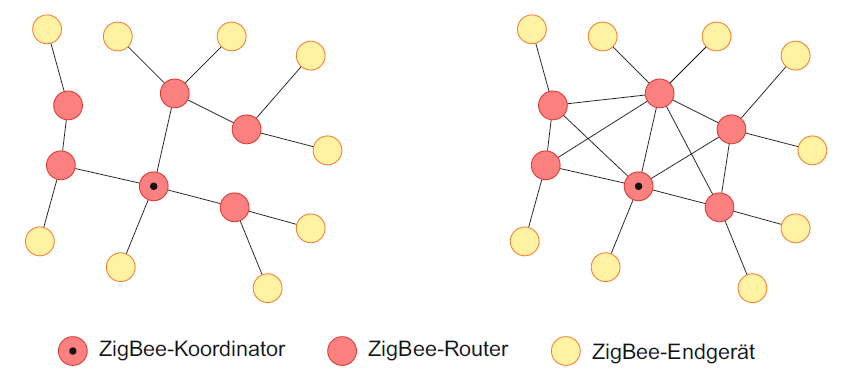
\includegraphics[width=0.8\textwidth]{Zigbee_Netztopologie.png}
	\caption{Zigbee Baumnetzwerk links und Meshnetzwerk rechts \cite[S.~221]{markus_krause_rainer_konrad_zigbee_2014}}	\label{fig:NetzwerktopologienZigbee}
\end{figure}

Wie in Abbildung \ref{fig:NetzwerktopologienZigbee} bereits angedeutet, kann innerhalb eines Zigbee Meshnetzwerkes zwischen drei Node Rollen unterschieden werden. Diese besitzen unterschiedliche Aufgaben und Eigenschaften und sind, wie nachfolgend beschrieben, spezifiziert:

\paragraph{Zigbee Koordinator}
Als zentrale Einheit übernimmt der \textit{Zigbee Koordinator}, Aufgaben wie den Aufbau und die Verwaltung eines WPAN (Wireless Personal Area Network). Dazu gehört die Definition der wichtigsten Parameter, wie die PAN-ID, die Sicherheitsschlüssel sowie die Wahl des IEEE Channels.
In einem Zigbee-Netzwerk gibt es genau ein Gerät, das die Rolle des \textit{Zigbee Koordinators} einnimmt.
Welches Gerät dies ist, wird vom Anwender respektive Entwickler bestimmt.
Wenn dieses Gerät das Netzwerk verlässt oder kurzzeitig ausser Betrieb ist, kann das Netzwerk zwar weiter bestehen und wie bisher betrieben werden. Für die Aufnahme von zusätzlichen Nodes oder für die Aktualisierung der Sicherheitsschlüssel, muss jedoch der \textit{Zigbee-Koordinator} wieder mit dem Netz verbunden werden.
Jeder \textit{Zigbee-Koordinator} besitzt gleichzeitig auch die Rolle eines \textit{Zigbee-Routers}. \cite{markus_krause_rainer_konrad_zigbee_2014}

\paragraph{Zigbee Router}
\textit{Zigbee-Router} bilden das eigentliche Meshnetzwerk, wie es in Abbildung \ref{fig:NetzwerktopologienZigbee} schematisch dargestellt ist.
Sie übernehmen die Aufgabe des Routings und leiten Pakete innerhalb des Netzwerkes weiter.
Durch Wegentdeckungsanfragen werden Routing-Tabellen aufgebaut und fortlaufend aktualisiert.
Diese Routing-Tabellen sind entscheidend für den gerouteten Versand von Datenpaketen.
\textit{Zigbee-Router} sind zudem potentielle Zugriffspunkte zum Netzwerk für \textit{Zigbee End-Devices}. \cite{markus_krause_rainer_konrad_zigbee_2014}

\paragraph{Zigbee End-Device}
Die einfachste Rolle in einem Zigbee Netzwerk ist jene des \textit{Zigbee End-Devices}. Das \textit{Zigbee End-Device} steht in einer Parent-Child-Beziehung mit einem \textit{Zigbee-Router}.
Diese Kommunikation findet entweder periodisch oder ausgelöst durch einen Userinput statt.
Ankommende Pakete werden jeweils vom Parent-Node gespeichert, bis das \textit{Zigbee End-Device} diese abruft.
\textit{Zigbee End-Devices} besitzen ausserdem keine Routing Funktionen und gelten deshalb als sehr energiesparend.
Ausgeführt als \textit{Sleepy-End-Device} können CPU und RAM des entsprechenden Nodes ganz oder teilweise heruntergefahren und durch periodische Interrupts geweckt werden.
Dadurch können noch längere Batteriestandzeiten erreicht werden.
In der Anwendung werden beispielsweise Lichtschalter als \textit{Sleepy-End-Device} ausgeführt, die keine draht­ge­bun­dene Energieversorgung besitzen. \cite{markus_krause_rainer_konrad_zigbee_2014}


\subsection{Zigbee Protokollstack}\label{subsec:ZigbeeProtokollStack}
Die Architektur des Zigbee Stacks besteht aus vier Layern, dem Physical Layer (PHY), dem Media Access Control Layer (MAC), dem Network Layer (NWK) und dem Application Layer (APL).
Abbildung \ref{fig:ArchitekturdesZigbeeProtokollStacks} zeigt den Aufbau des Protokollstacks.
Jede der Schichten ist mit bestimmten Aufgaben betraut und stellt der darüber liegenden Schicht die notwendigen Daten und Dienste zur Verfügung.
Nachfolgend wird auf die vier Schichten des Zigbee Stacks, einzeln eingegangen und deren Aufgabe und Funktionsweise kurz erläutert.

\begin{figure}[h]
	\centering
	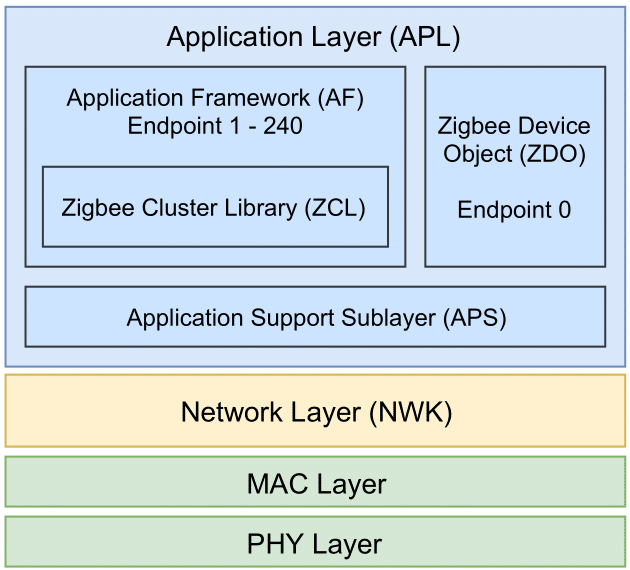
\includegraphics[width=0.5\textwidth]{Zigbee_Architektur.png}
	\caption{Architektur des Zigbee Protokollstacks}
	\label{fig:ArchitekturdesZigbeeProtokollStacks}
\end{figure}

\subsubsection{MAC und PHY Layer}\label{subsubsec:MACundPHYLayer}
Der MAC wie auch der PHY Layer werden im Zigbee Protokollstack gebildet, durch den \textit{IEEE 802.15.4} Standard für \textit{Wireless Personal Area Networks (WPAN)}.
Während beispielsweise Wifi oder Bluetooth, die auf dem selben 2.4 GHz ISM-Funkfrequenzband betrieben werden können, für hohe Datenübertragungsraten konzipiert wurden, ist dieser Standard für kleinere Datenmengen optimiert.
Durch die Vermeidung von unnötigen Steuerinformationen kann der \textit{IEEE 802.15.4} Standard auf einfachster Hardware realisiert und mit kleinstem Energieaufwand betrieben werden.
Dies ist ideal für sogenannte \textit{Wireless Sensor Networks (WSN)}.
Zigbee ist dabei nur eines von vielen Protokollen, die diesen Standard benutzen.
MAC und PHY Layer sind für die physikalische Datenübertragung von einem zum anderen Node zuständig.
Dazu besitzt jedes Funkmodul eine einmalige 48-Bit MAC Adresse, mit welcher das Gerät eindeutig identifiziert und adressiert werden kann. \cite{markus_krause_rainer_konrad_ieee_2014}


\subsubsection{Network Layer (NWK)}\label{subsubsec:Network Layer}
Der NWK Layer ist im Zigbee Stack für den Aufbau, das Management der Netzwerkfunktionen sowie das Routing innerhalb dieses Netzwerkes verantwortlich.
Im NWK Layer wird das eigentliche Mesh gebildet und unterhalten.

\paragraph{Netzaufbau und Adressierung}
Wie unter \ref{subsec:ZigbeeNetzaufbauundTopologie} bereits erwähnt, ist der Koordinator verantwortlich für den Aufbau des Zigbee Netzwerks und die Wahl von entsprechend geeigneten Parametern.
Dazu gehört beispielsweise eine 16-Bit PAN-ID sowie die Wahl eines möglichst störungsfreien Funkkanals.
Beim Beitritt eines neuen Funkmoduls, wird diesem durch den Koordinator eine im Netzwerk einmalige 16-Bit \textit{Short-Address} zugewiesen.
Anhand dieser Adresse kann das Funkmodul nun im Netzwerk adressiert werden und das Funkmodul selbst kann damit Routing Funktionen wahrnehmen.
Die im MAC Layer definierte 48-Bit MAC Adresse wird im NWK Layer in eine statische 64-Bit \textit{Long-Address} umgewandelt.
Letztere kann im Zigbee Stack ebenfalls für die Adressierung verwendet werden.
In einer \textit{Address-Table} sind die statischen \textit{Long-Addresses} und die dynamischen \textit{Short-Addresses} einander eindeutig zugewiesen.
Für die Adressierung im NWK Layer und für das Routing wird ausschliesslich die \textit{Short-Address} verwendet.

\paragraph{Routing}
Innerhalb von Zigbee Mesh Netzwerken, welche das \textit{ZigBee PRO}-Stackprofil verwenden, werden durch jeden \textit{Zigbee-Router} Routingtabellen erstellt.
Falls sich das Netzwerk verändert, werden auch diese Routing-Tabellen nachgeführt.
In den Routing-Tabellen ist die \textit{Short-Address} des Zielnodes sowie die zugehörige \textit{Next-Hop-Address} zum Ziel hinterlegt.
Eine zentrale Einheit, die das Routing übernimmt, gibt es nicht.
Enthält die Routingtabelle veraltete Einträge oder sind für das entsprechende Ziel noch keine Informationen vorhanden, muss ein \textit{Route Discovery} durchgeführt werden.
Hierbei handelt es sich um eine Broadcast Nachricht, welche an alle Router gesendet wird.
Die Router in unmittelbarer Umgebung empfangen die Nachricht und leiten sie als Broadcast an alle Router in ihrer Reichweite weiter.
Dabei werden die Wegkosten jeweils addiert, um diese, sobald die Nachricht beim Zielnode angekommen ist, dem Absender mitzuteilen.
Auf diese Weise wird der Weg mit den geringsten totalen Wegkosten ermittelt und in der Routingtabelle abgelegt.


\subsubsection{Application Layer (APL)}\label{subsubsec:ApplicationLayer}
Der Zigbee Application Layer kann in drei Teile unterteilt werden, den Application Support Sublayer, das Zigbee Device Object und das Application Framework mit der Zigbee Cluster Library, in der die eigentliche Anwendung definiert ist.

\paragraph{Application Support Sublayer (APS)}
Wie der Name andeutet, ist der APS Layer für die Anwendungsunterstützung zuständig und als Zwischenschicht im Application Layer eingebettet.
Zu den Aufgaben des APS Layers gehören das \textit{Binding}, das \textit{Group-Management}, die Datenübertragung inkl. Fragmentierung sowie die Erstellung und der Versand von APS-Frames.
Ausserdem bietet der APS Layer die Möglichkeit der Empfangsbestätigung auf Applikationsebene.
Anders als die Empfangsbestätigung auf MAC Ebene ist diese nicht nur auf Funkmodule in unmittelbarer Reichweite beschränkt.

\begin{figure}[h]
	\centering
	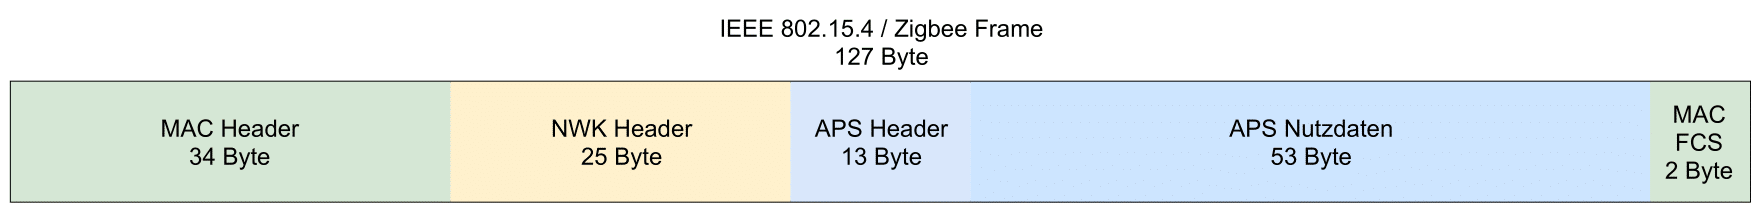
\includegraphics[width=\textwidth]{Zigbee_Frame_Structure.png}
	\caption{Zigbee Frame Struktur bei aktivierten Sicherheitsfunktionen \cite[S.~286]{markus_krause_rainer_konrad_zigbee_2014}}
	\label{fig:ZigbeeFrameStruktur}
\end{figure}

Die Fragmentierung von APS Nutzdaten basiert darauf, dass die Grösse von Frames durch den PHY Layer auf 127 Byte beschränkt ist.
Abzüglich sämtlicher Header auf MAC, NWK sowie APS Ebene und sonstigem Overhead des Protokolls, beispielsweise von Sicherheitsfunktionen (siehe Abschnitt \ref{subsucsec:ZigbeeSicherheit}), reduziert sich die nutzbare APS-Payload Grösse auf 53 Byte. In Abbildung \ref{fig:ZigbeeFrameStruktur} ist die Struktur eines kompletten Zigbee Frames dargestellt.
Sollen nun grössere Daten übertragen werden, führt der APS Layer eine Fragmentierung durch. \cite[S.~279 - 299]{markus_krause_rainer_konrad_zigbee_2014}


\paragraph{Application Framework (AF) mit Zigbee Cluster Library (ZCL)}
Das Application Framework bildet den Bereich des APL, in dem die eigentliche Anwendung abläuft. Für die Adressierung stehen dem Anwender dabei 240 sogenannte Endpoints zur Verfügung. Endpoints können mit dem Prinzip von Ports im TCP/IP Modell verglichen werden.
Sie dienen dazu unterschiedliche Anwendungen auf dem selben Node zu adressieren.
Innerhalb des AF können Anwendungen nun prinzipiell frei umgesetzt werden.
Um den Anwendern jedoch eine herstellerunabhängige Plattform bieten zu können, wurde durch die Zigbee Alliance die \textit{Zigbee Cluster Library (ZCL)} spezifiziert.
Anwendungen wie beispielsweise ein Lichtschalter oder eine Lampe werden durch sogenannte Cluster detailliert beschrieben.
Dabei handelt es sich um eine Sammlung von Kommandos und Attributen für den jeweiligen Anwendungszweck. \cite{the_zigbee_alliance_zigbee_2016}

\paragraph{Zigbee Device Object (ZDO)}
Das Zigbee Device Object ist ein eigenständiges Anwendungsobjekt, welches immer mit dem Endpoint 0 adressiert wird.
Es setzt die Funktionalitäten gemäss Definition der Zigbee Rollen (Koordinator, Router, End-Device) um und benutzt dafür Funktionen der NWK sowie APS Schicht.
Beispielsweise ist es zuständig für das Netzwerkmanagement, Knotenmanagement und für die Implementation von Sicherheitsfunktionen.

\subsubsection{Sicherheit}\label{subsucsec:ZigbeeSicherheit}
Die drahtlose Übertragung in einem WPAN ist vom Grundsatz her anfälliger für Angriffe oder Manipulationen wie eine drahtgebun­dene Kommunikation.
Deshalb ist die Implementation von Sicherheitsfeatures in einem \textit{Low Power Mesh Network} von grosser Bedeutung.
Zigbee verwendet ein \textit{CCM\footnote{Counter mode encryption and Cipher block chaining Message authentication code}} Verfahren auf MAC wie auch auf NWK und APS Ebene.
Dieses ist vom \textit{IEEE 802.15.4} Standard für die Verschlüsselung und Authentifizierung spezifiziert.
\textit{CCM} ist ein Verfahren für eine mehrmalige Blockverschlüsselung, welches mit einem einzigen Schlüssel auskommt.
Das Verfahren nutzt den \textit{AES\footnote{Advanced Encryption Standard}}-Verschlüsselungsalgorithmus als Blockverschlüsselung.

\paragraph{Sicherheitsstufen}
Im \textit{CCM} Verfahren können acht verschiedene Sicherheitsstufen gemäss Tabelle \ref{tab:SicherheitsstufeninZigbee} definiert werden.
Die Sicherheitsstufe 0 deaktiviert sämtliche Sicherheitsfunktionen.
Die Stufen 1 bis 3 fügen dem MAC Frame eine \textit{MIC\footnote{Message Integrity Code}} Prüfsumme von steigender Grösse hinzu, wodurch die Grösse des Frames zunimmt.
Erst ab Stufe 4 werden die Nutzdaten des MAC-Frames verschlüsselt und die Stufen 5 bis 7 mit einer \textit{MIC} Prüfsumme ergänzt. \cite[S.~334]{markus_krause_rainer_konrad_zigbee_2014}

\begin{table}[h]
\centering
\begin{tabular}{lll} 
\toprule
Sicherheitsstufe: & Verschlüsselung: & Authentifikation: \\ 
\hline
0 & Nein & Nein \\
1 & Nein & 32-Bit \textit{MIC} \\
2 & Nein & 64-Bit~\textit{MIC} \\
3 & Nein & 128-Bit~\textit{MIC} \\
4 & Ja & Nein \\
5 & Ja & 32-Bit~\textit{MIC} \\
6 & Ja & 64-Bit~\textit{MIC} \\
7 & Ja & 128-Bit~\textit{MIC} \\
\bottomrule
\end{tabular}
\caption{Sicherheitsstufen im Zigbee Protokollstack \cite[S.~334]{markus_krause_rainer_konrad_zigbee_2014}}
\label{tab:SicherheitsstufeninZigbee}
\end{table}

\paragraph{Schlüssel}
Für das \textit{CCM} Verfahren in Zigbee Netzwerken werden zwei verschiedene Schlüsseltypen eingesetzt, der Netzwerkschlüssel und der sogenannte Linkschlüssel.
In einem Zigbee Netzwerk mit normalem Sicherheitsmodus\footnote{Die Alternative zum \textit{Normalen Sicherheitsmodus} wäre der \textit{Hohe Sicherheitsmodus}. \cite[S.~338]{markus_krause_rainer_konrad_zigbee_2014}} wird einem Node die Rolle des \textit{Trustcenters} zugeordnet.
Üblicherweise übernimmt diese Rolle der \textit{Zigbee-Koordinator}.
Der Trustcenter-Node ist zuständig für die Verteilung der Sicherheitsschlüssel.
Beim Beitritt eines Nodes zum Netzwerk überträgt das \textit{Trustcenter} den Netzwerkschlüssel über einen unverschlüsselten Kanal.
Dieser Netzwerkschlüssel wird nun für die Kommunikation zwischen Node und \textit{Trustcenter} benutzt.
Um Angriffe zu verhindern, wird der Netzwerkschlüssel durch das \textit{Trustcenter} regelmässig erneuert.
Dazu werden sogenannte Schlüsselwechsel-Kommandoframes versendet.
Für die Verschlüsselung von End-zu-End Verbindungen auf APS Ebene werden Linkschlüssel eingesetzt, welche nur über die bereits gesicherte Verbindung vom Trustcenter zum Node übertragen werden.
Diese Linkschlüssel sind nur den beteiligten Nodes bekannt und werden üblicherweise durch das \textit{Trustcenter} ausgestellt.
Eine Alternative dazu wäre, die Linkschlüssel auf den entsprechenden Funkmodulen bereits vor zu installieren.

